
\begin{figure}[t!]
  \begin{minipage}[b]{.23\textwidth}
    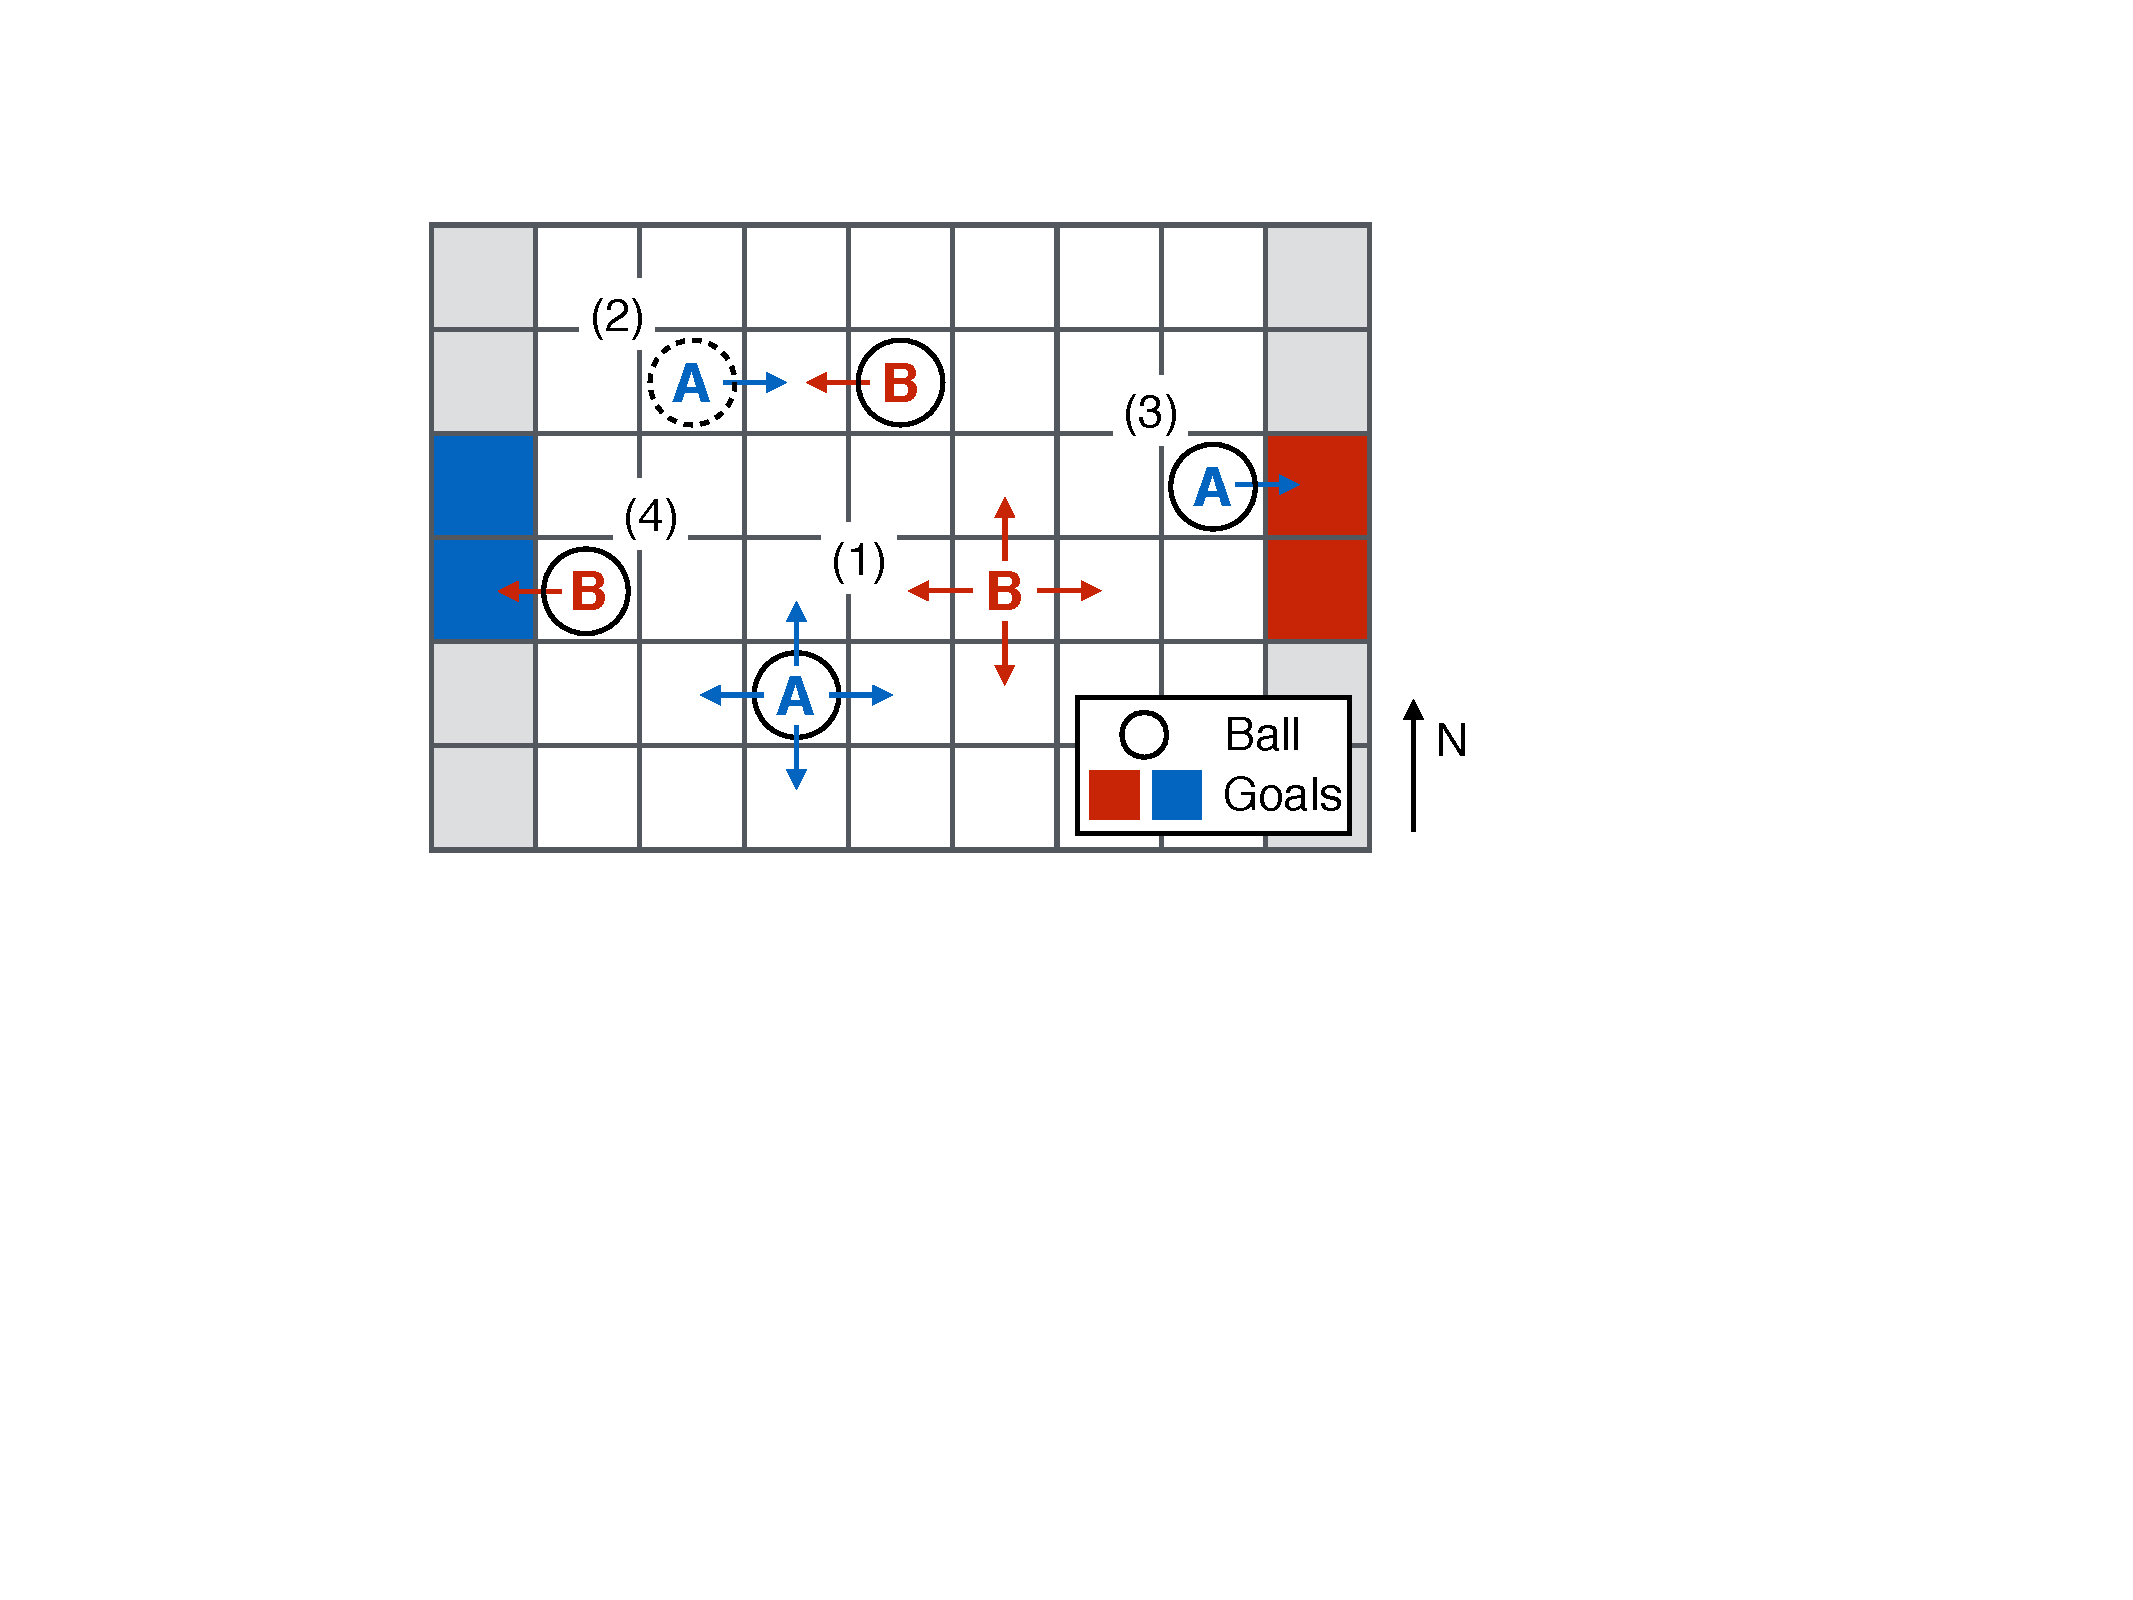
\includegraphics[width=1\linewidth]{2016_icml_opponent/figures/soccer_illustration}
  \end{minipage}
  \begin{minipage}[b]{.23\textwidth}
    \setlength{\tabcolsep}{1.5pt}
    \renewcommand{\arraystretch}{0.7}
    \begin{tabular}[b]{ccc}
      \toprule
      & Defensive & Offensive \\
      \midrule
      \multirow{2}{*}{w/ ball} & Avoid & Advance \\
      & opponent & to goal \vspace{2pt} \\
      \midrule\vspace{2pt}
      \multirow{2}{*}{w/o ball} & Defend & Intercept \\
      & goal & the ball \\
      \bottomrule
    \end{tabular}
  \end{minipage}
  \caption{\emph{Left:} Illustration of the soccer game.
    \emph{Right:} Strategies of the hand-crafted rule-based agent.}
  \label{fig:soccer_game}
\end{figure}


\section{Experiments}
\label{sec:experiments}

In this section, we evaluate our models on two tasks, the soccer game
and quiz bowl.  Both tasks have two players against each other and the
opponent presents varying behavior.  We compare \dron{} models with
\dqn{} and analyze their response against different types of
opponents.

All systems are trained under the same Q-learning framework.  Unless
stated otherwise, the experiments have the following
configuration: discount factor $\gamma$ is 0.9, parameters are optimized by AdaGrad~\cite{duchi2011adaptive} with a learning rate of 0.0005, and the mini-batch size is 64.  We use
$\epsilon$-greedy exploration during training, starting with an
exploration rate of 0.3 that linearly decays to 0.1 within 500,000
steps.  We train all models for fifty epochs.
Cross Entropy is used as the loss in multitasking learning.

\subsection{Soccer}

Our first testbed is a soccer variant following previous work on
multi-player
games~\cite{minimax-q,collins-thesis-rl,opponent-qlearning}.  The game
is played on a $6\times 9$ grid (Figure~\ref{fig:soccer_game}) by two
players, A and B.\footnote{Although the game is played in a grid
  world, we do not represent the $Q$-function in tabular form as in
  previous work. Therefore it can be generalized to more complex
  pixel-based settings.}  The game starts with A and B in a
randomly squares in the left and right half (except the
goals), and the ball goes to one of them.  Players choose
from five actions: \act{move N, S, W, E} or \act{stand} still
(Figure~\ref{fig:soccer_game}(1)).  An action is invalid if it takes
the player to a shaded square or outside of the border.  If two
players move to the same square, the player who possesses the ball
before the move loses it to the opponent
(Figure~\ref{fig:soccer_game}(2)), and the move does not take place.


A player scores one point if they take the ball
to the opponent's goal (Figure~\ref{fig:soccer_game}(3), (4)) and the
game ends.  If neither player gets a goal within one hundred steps,
the game ends with a zero--zero tie.

\paragraph{Implementation}

We design a two-mode rule-based agent as the opponent Figure~\ref{fig:soccer_game}(right).
In the offensive mode, the agent always prioritize
attacking over defending.  In 5000 games against a random agent, it wins 99.86\%
of the time and the average episode length is 10.46.
In defensive mode, the agent only
focuses on defending its own goal.  As a result, it wins 31.80\% of the games
and ties 58.40\% of them; the average episode length is 81.70.
It is easy to find a strategy to defeat the opponent in either mode,
however, the strategy does not work well for both modes, as we will show in Table~\ref{tab:soccer_matrix}.
Therefore, the agent randomly chooses between the two modes in each game to create a varying strategy.

The input state is a $1\times 15$ vector representing coordinates of
the agent, the opponent, the axis limits of the field, positions of
the goal areas and ball possession.  We define a player's move
by five cases: approaching the agent, avoiding the agent, approaching the agent's goal,
approaching self goal and standing still.  Opponent features
include frequencies of observed opponent moves, its most recent move
and action, and the frequency of losing the ball to the opponent.

The baseline \dqn{} has two hidden layers, both with 50 hidden units.
We call this model \dqn{}-world: opponents are modeled as
part of the world.  The hidden layer of the opponent network in
\dron{} also has 50 hidden units.  For multitasking, we experiment
with two supervision signals, opponent action in the current state
(+action) and the opponent mode (+type).

\paragraph{Results}
\begin{table}

\centering
\begin{tabular}[ht]{lccc}
\toprule
\multirow{2}{*}{Model} & \multirow{2}{*}{Basic} & \multicolumn{2}{c}{Multitask} \\
& & +action & +type \\
\midrule
\multicolumn{4}{c}{Max $R$} \\
\midrule
\dron{}-concat & 0.682 & 0.695$^\ast$ & 0.690$^\ast$ \\
\dronmoe{} & {\bf 0.699}$^\ast$ & 0.697$^\ast$ & 0.686$^\ast$ \\
\dqn{}-world & 0.664 & - & - \\
\midrule
\multicolumn{4}{c}{Mean $R$} \\
\midrule
\dron{}-concat & 0.660 & 0.672 & 0.669 \\
\dronmoe & 0.675  & 0.664 & 0.672 \\
\dqn{}-world & 0.616 & - & - \\
\bottomrule
\end{tabular}
\caption{
  Rewards of \dqn{} and \dron{} models on Soccer.
  We report the maximum test reward ever achieved (Max $R$) and
  the average reward of the last 10 epochs (Mean $R$).
  Statistically significant ($p<0.05$ in two-tailed pairwise
  $t$-tests) improvement for \dqn{} ($^\ast$) and all other
  models in {\bf bold}. \dron{} models achieve higher rewards in both measures.
}

\label{tab:soccer_model_result}
\end{table}

In Table~\ref{tab:soccer_model_result}, we compare rewards of \dron{}
models, their multitasking variations, and \dqn{}-world.  After each
epoch, we evaluate the policy with 5000 randomly generated games (the test set) and
compute the average reward.  We report the mean test reward after the
model stabilizes and the maximum test reward ever achieved.  The
\dron{} models outperform the \dqn{} baseline.  Our model also has much
smaller variance (Figure~\ref{fig:soccer_all_test_rewards}).

Adding additional
supervision signals improves \dron-concat but not \dronmoe\ (multitask column).
\dron-concat does not explicitly learn
different strategies for different types of opponents, therefore more
discriminative opponent representation helps model the relation
between opponent behavior and Q-values.  However, for \dronmoe,
while better opponent representation is still desirable, the
supervision signal may not be aligned with ``classification'' of the
opponents learned from the Q-values.

\begin{figure}
\centering
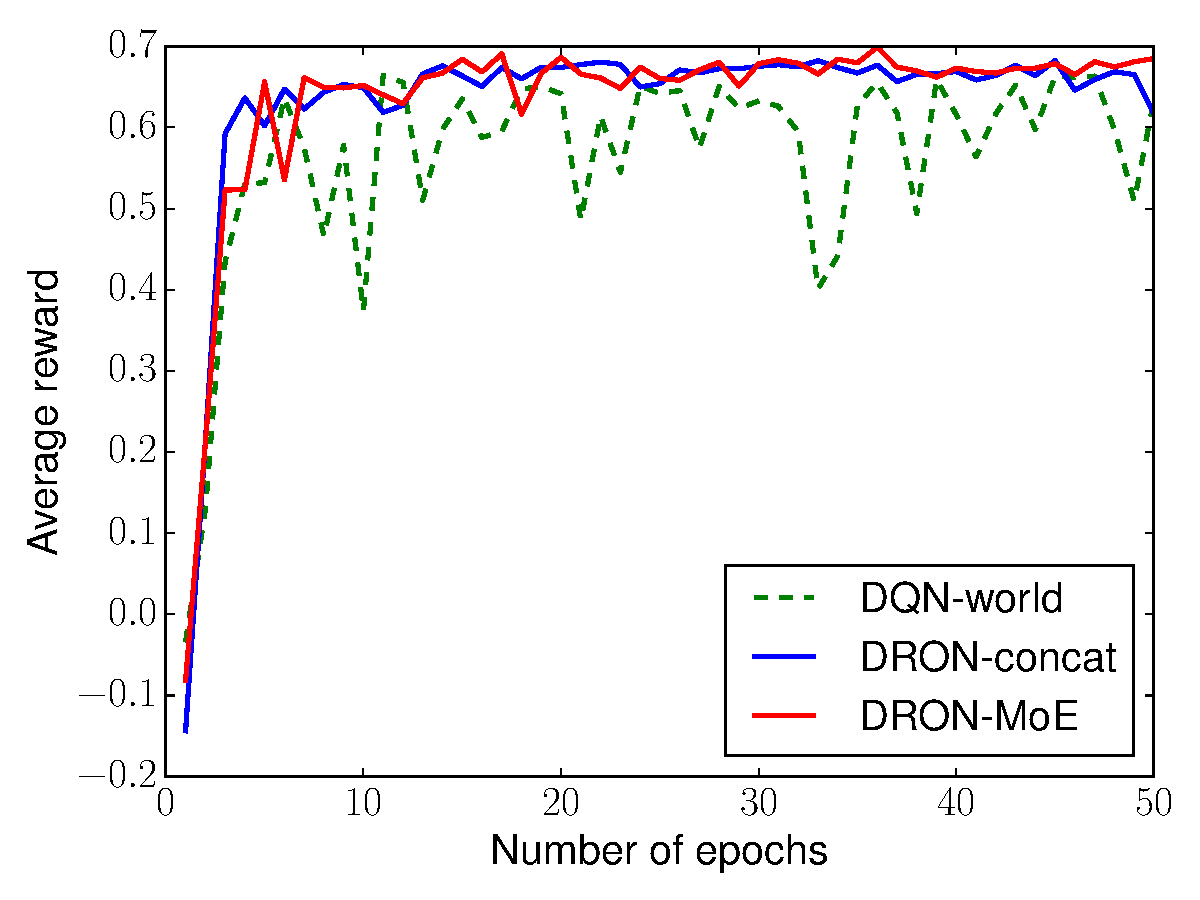
\includegraphics[width=0.6\linewidth]{2016_icml_opponent/figures/soccer_all_test_rewards}
\caption{Learning curves on Soccer over fifty epochs. \dron{} models are
  more stable than \dqn{}.}
\label{fig:soccer_all_test_rewards}
\end{figure}

\begin{table}[t!]
\centering
\begin{tabular}{cccccc}
\toprule
& \multicolumn{2}{c}{\dqn{}} & \dqn{}& \dron{} & \dron{} \\
& O only & D only & -world & -concat & -\abr{moe} \\
\midrule
O & {\bf 0.897} & -0.272 & 0.811 & 0.875 & 0.870 \\
D & 0.480 & {\bf 0.504} & 0.498 & 0.493 & 0.486 \\
\bottomrule
\end{tabular}
\caption{Average rewards of \dqn{} and \dron{} models when playing against different types of opponents. Offensive and defensive agents are represented by O and D. ``O only'' and ``D only'' means training against O and D agents only. Upper bounds of rewards are in bold. \dron{} achieves rewards close to the upper bounds against both types of opponents.}
\label{tab:soccer_matrix}
\end{table}

To investigate how the learned policies adapt to different opponents,
we test the agents against a defensive opponent and an offensive
opponent separately.  Furthermore, we train two \dqn{} agents targeting
at each type of opponent respectively.
Their performance is best an agent can do when facing a single type of opponent (in our setting),
as the strategies are learned to defeat this particular opponent.
Table~\ref{tab:soccer_matrix} shows the
average rewards of each model and the \dqn{} upper bounds (in bold).  \dqn{}-world is confused
by the defensive behavior and significantly sacrifices its performance
against the offensive opponent; \dron{} achieves a much better
trade-off, retaining rewards close to both upper bounds against the
varying opponent.

\begin{figure}[t]
\centering
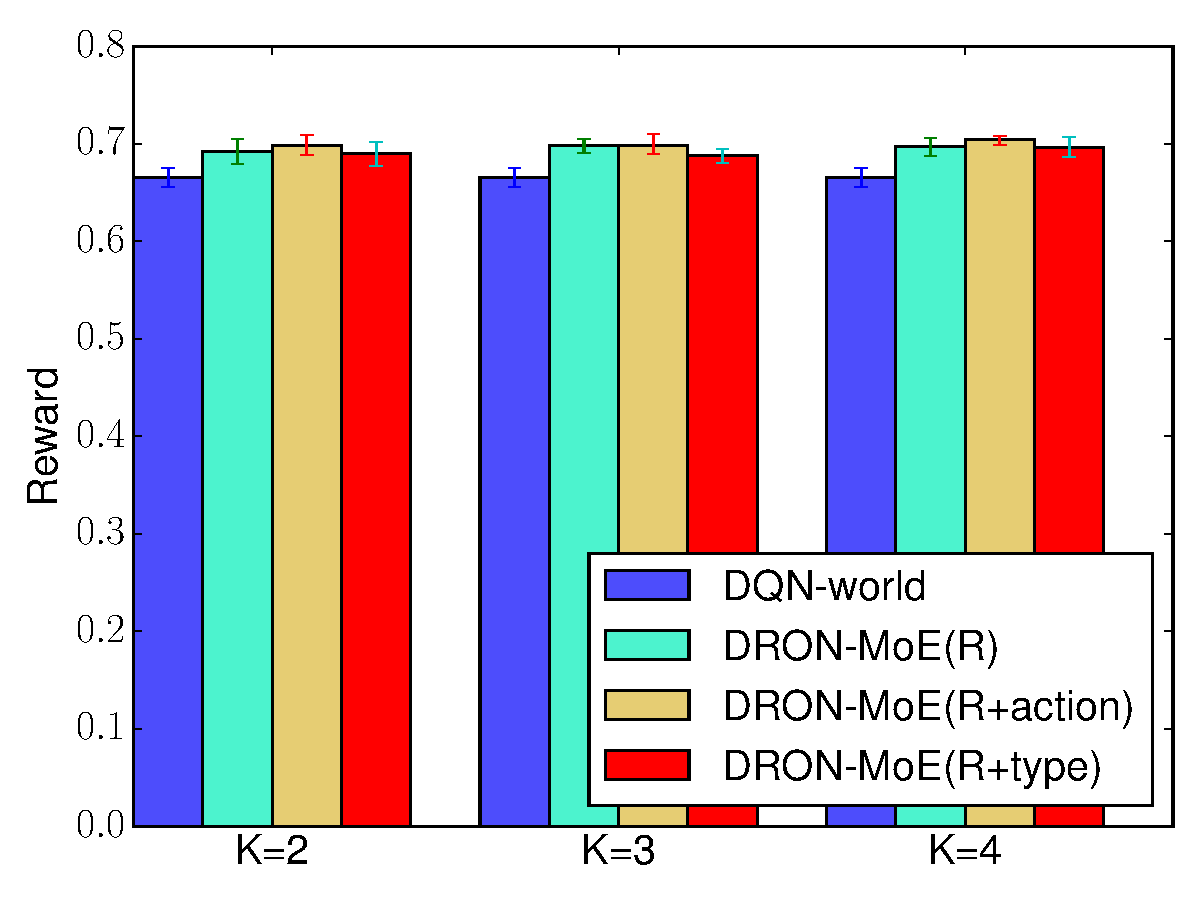
\includegraphics[width=0.6\linewidth]{2016_icml_opponent/figures/soccer_moe_bar}
\caption{Effect of varying the number experts (2--4) and multitasking on Soccer.
The error bars show the 90\% confidence interval.
\dronmoe{} consistently improves over DQN regardless of the number of mixture components.
Adding extra supervision does not obviously improve the results.
}
\label{fig:soccer_moe_bar}
\end{figure}

Finally, we examine how the number of experts in \dronmoe{} affects
the result. From Figure~\ref{fig:soccer_moe_bar}, we see no
significant difference in varying the number of experts, and
\dronmoe{} consistently performs better than \dqn{} across all $K$.
Multitasking does not help here.

\subsection{Quiz Bowl}

Quiz bowl is a trivia game widely played in English-speaking countries between
schools, with tournaments held most
weekends. It is usually played between two
teams.  The questions are read to players and they score points by ``buzzing in''
first (often before the question is finished) and answering the question
correctly.
One example question with buzzes is shown in Figure~\ref{fig:buzz_example}.
A successful quiz bowl player needs two things: a content
model to predict answers given (partial) questions and a buzzing model to decide
when to buzz.

\paragraph{Content Model}

We model the question answering part as an incremental text-classification
problem.  Our content model is a recurrent neural network with gated recurrent
units (\gru{}).  It reads in the question sequentially and outputs a distribution
over answers at each word given past information encoded in the hidden states.

\paragraph{Buzzing Model}

To test depth of knowledge, questions start
with obscure information and reveals more and more obvious clues towards the
end (e.g., Figure~\ref{fig:buzz_example}).  Therefore, the buzzing model faces a speed-accuracy tradeoff: while
buzzing later increases one's chance of answering correctly, it also increases
the risk of losing the chance to answer.  A safe strategy is to always buzz as
soon as the content model is confident enough.  A smarter strategy, however, is
to adapt to different opponents: if the opponent often buzzes late, wait for more clues; otherwise, buzz more aggressively.

To model interaction with other players, we take a reinforcement learning
approach to learn a buzzing policy.  The state includes words revealed and
predictions from the content model, and the actions are \act{buzz} and
\act{wait}.  Upon buzzing, the content model outputs the most likely answer at
the current position.  An episode terminates when one player buzzes and answers
the question correctly.  Correct answers are worth 10 points and wrong answers
are $-5$.

\begin{figure}[t]
\centering
\subfigure[]{
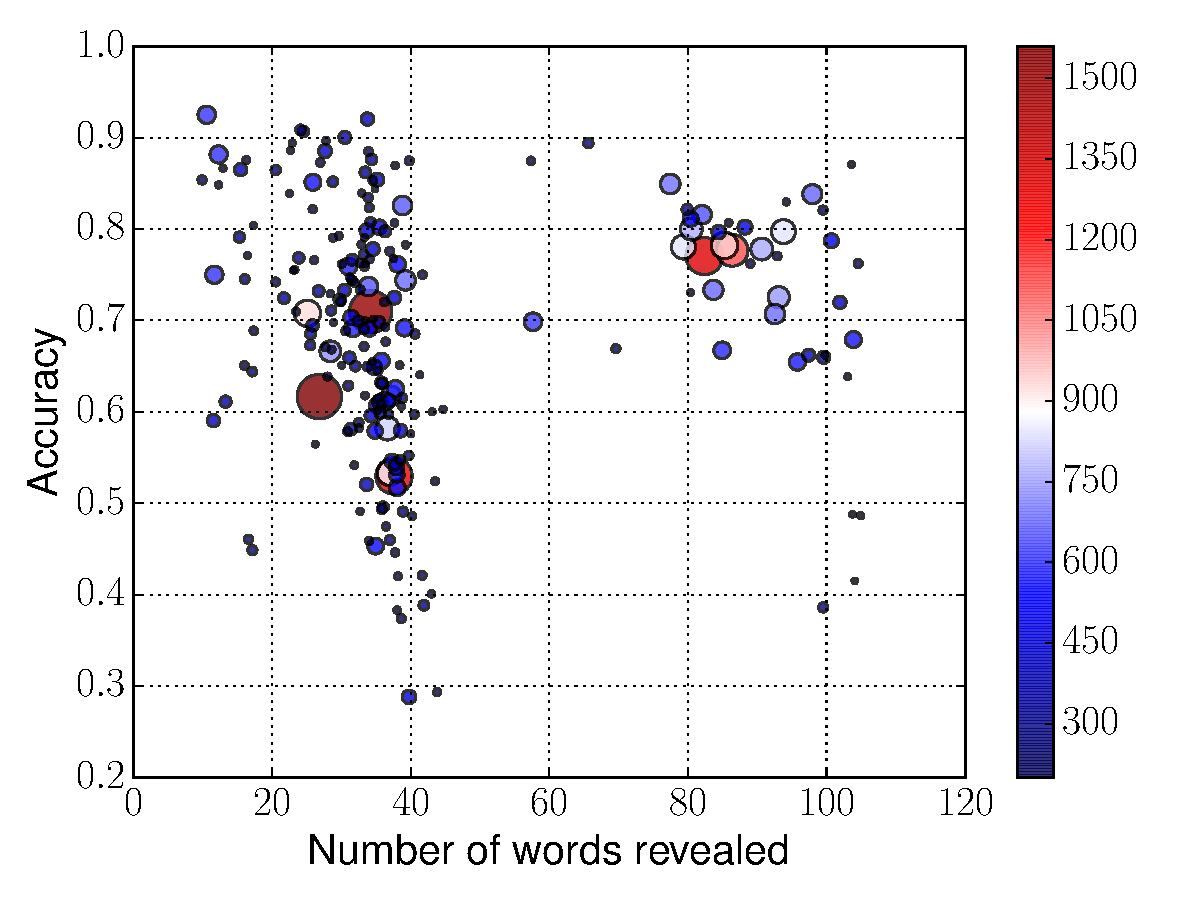
\includegraphics[width=0.23\textwidth]{2016_icml_opponent/figures/acc_pos_scatter}
\label{fig:player_acc}
}
\hspace{-1em}
\subfigure[]{
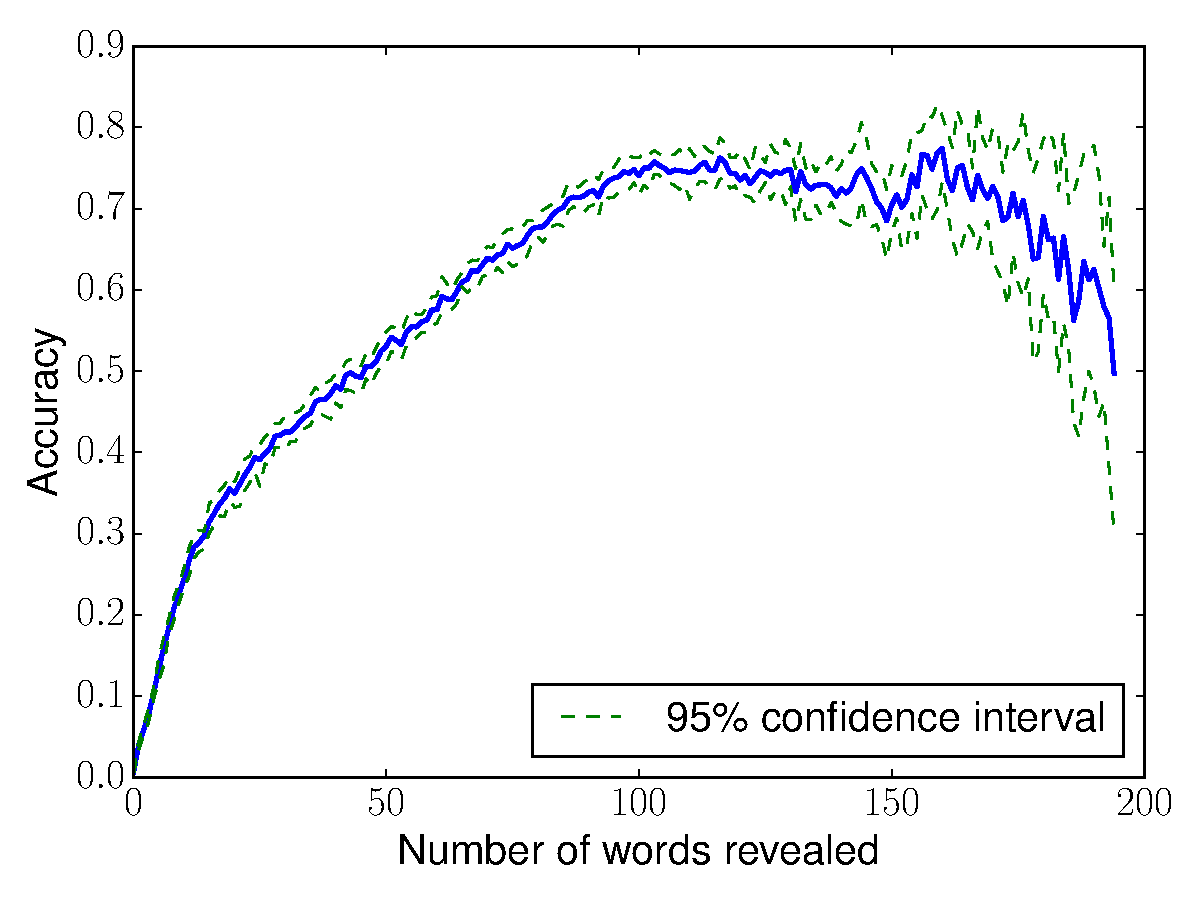
\includegraphics[width=0.23\textwidth]{2016_icml_opponent/figures/content_acc}
\label{fig:content_model_acc}
}
\caption{Accuracy vs. the number of words revealed. (a) Real-time user
  performance. Each dot represents one user; dot size and color correspond to
  the number of questions the user answered. (b) Content model
  performance. Accuracy is measured based on predictions at each word.
  Accuracy improves as more words are revealed.}
\end{figure}

\paragraph{Implementation}

We collect question/answer pairs and log user buzzes from Protobowl, an online
multi-player quizbowl application.\footnote{\url{http://protobowl.com}}
Additionally, we include data from
\citet{Boyd-Graber:Satinoff:He:Daume-III-2012}.
Most buzzes are from strong tournament players.
After removing answers with
fewer than five questions and users who played fewer than twenty questions, we end up with
1045 answers and 37.7k questions.  We divide all questions into two
non-overlapping sets: one for training the content model and one for training
the buzzing policy.
The two sets are further divided into train/dev and train/dev/test sets randomly.
There are clearly two clusters of players
(Figure~\ref{fig:player_acc}): aggressive players who buzz early with varying
accuracies and cautious players who buzz late but maintain higher accuracy.
Our \gru{} content model (Figure~\ref{fig:content_model_acc}) is more accurate
with more input words---a behavior similar to human players.

Our input state must represent information from the content model and the
opponents.  Information from the content model takes the form of a \emph{belief
  vector}: a vector ($1\times 1045$) with the current estimate (as a log probability) of
each possible guess being the correct answer given our
input so far. We concatinate the belief vector from the previous time
step to capture sudden shifts in certainty, which are
often good opportunities to buzz.
In addition, we include the number of words seen and whether a wrong buzz has happened.

The opponent features include the number of questions the opponent has answered,
the average buzz position, and the error rate.  The basic \dqn{} has two hidden
layers, both with 128 hidden units.  The hidden layer for the opponent has ten
hidden units.  Similar to soccer, we experiment with two settings for
multitasking: (a) predicting how opponent buzzes; (b)
predicting the opponent type.  We approximate the ground truth for
(a) by $\min(1, t/\mbox{buzz position})$ and use the mean square error as the
loss function.  The ground truth for (b) is based on dividing players into four
groups according to their buzz positions---the percentage of question
revealed.

\begin{table*}[t]
\setlength{\tabcolsep}{1.5pt}

\begin{tabular}{lccc@{\hskip 3ex}ccc@{\hskip 3ex}ccc@{\hskip 3ex}ccc@{\hskip 3ex}ccc}
\toprule
\multirow{3}{*}{Model} & \multirow{2}{*}{Basic} & \multicolumn{2}{c}{Multitask} & \multicolumn{12}{c}{Basic vs. opponents buzzing at different positions (\%revealed (\#episodes))} \\
& & +action & +type & \multicolumn{3}{c}{\hspace{-3ex}$0-25\%$ (4.8k)} & \multicolumn{3}{c}{\hspace{-2ex}$25-50\%$ (18k)} & \multicolumn{3}{c}{\hspace{-2ex}$50-75\%$ (0.7k)} & \multicolumn{3}{c}{$75-100\%$ (1.3k)}  \\
\cmidrule(lr){2-4}\cmidrule(lr){5-16}
& \multicolumn{3}{c}{$R\uparrow$} & $R\uparrow$ & rush$\downarrow$ & miss$\downarrow$ & $R\uparrow$ & rush$\downarrow$ & miss$\downarrow$ & $R\uparrow$ & rush$\downarrow$ & miss$\downarrow$ & $R\uparrow$ & rush$\downarrow$ & miss$\downarrow$ \\
\midrule
\dron{}-concat & 1.04 & {\bf 1.34}$^\ast$ & {\bf 1.25} & -0.86 & 0.06 & 0.15 & 1.65 & 0.10 & 0.11 & -1.35 & 0.13 & 0.18 & 0.81 & 0.19 & 0.12 \\
\dronmoe{} & {\bf 1.29}$^\ast$ & 1.00 & {\bf 1.29}$^\ast$ & -0.46 & 0.06 & 0.15 & 1.92 & 0.10 & 0.11 & -1.44 & 0.18 & 0.16 & 0.56 & 0.22 & 0.10 \\
\dqn{}-world & 0.95 & - & - & -0.72 & 0.04 & 0.16 & 1.67 & 0.09 & 0.12 & -2.33 & 0.23 & 0.15 & -1.01 & 0.30 & 0.09 \\
\dqn{}-self & 0.80 & - & - & -0.46 & 0.09 & 0.12 & 1.48 & 0.14 & 0.10 & -2.76 & 0.30 & 0.12 & -1.97 & 0.38 & 0.07 \\
\bottomrule
\end{tabular}

\caption{Comparison between \dron{} and \dqn{} models. The left column shows the average reward of each model on the test set. The right column shows performance of the basic models against different types of players, including the average reward ($R$), the rate of buzzing incorrectly (rush) and the rate of missing the chance to buzz correctly (miss). $\uparrow$ means higher is better and $\downarrow$ means lower is better.
  In the left column, we indicate statistically significant results ($p<0.05$ in two-tailed pairwise $t$-tests) with boldface for vertical comparison and $^\ast$ for horizontal comparison.}
\label{tab:model_result}
\end{table*}


\paragraph{Results}

In addition to \dqn{}-world, we also compare with \dqn{}-self, a
baseline without interaction with opponents at all. \dqn{}-self is
ignorant of the opponents and plays the safe strategy:
answer as soon as the content model is confident.  During training, when the answer
prediction is correct, it receives reward 10 for \act{buzz} and -10 for
\act{wait}.  When the answer prediction is incorrect, it receives
reward -15 for \act{buzz} and 15 for \act{wait}.  Since all rewards
are immediate, we set $\gamma$ to 0 for \dqn{}-self.\footnote{This is equivalent to cost-sensitive classification.}
With data of the
opponents' responses, \dron{} and \dqn{}-world use the game payoff
(from the perspective of the computer) as the reward.

 

First we compare the average rewards on test set of our models---\dron{}-concat
and \dronmoe{} (with 3 experts)---and the baseline models: \dqn{}-self and
\dqn{}-world.  From the first column in Table~\ref{tab:model_result}, our models
achieve statistically significant improvements over the \dqn{} baselines and
\dronmoe{} outperforms \dron{}-concat.
In addition, the \dron{} models have much less variance compared to \dqn{}-world as the learning curves show in Figure~\ref{fig:qb_all_test_rewards}.


\begin{figure}[t]
\centering
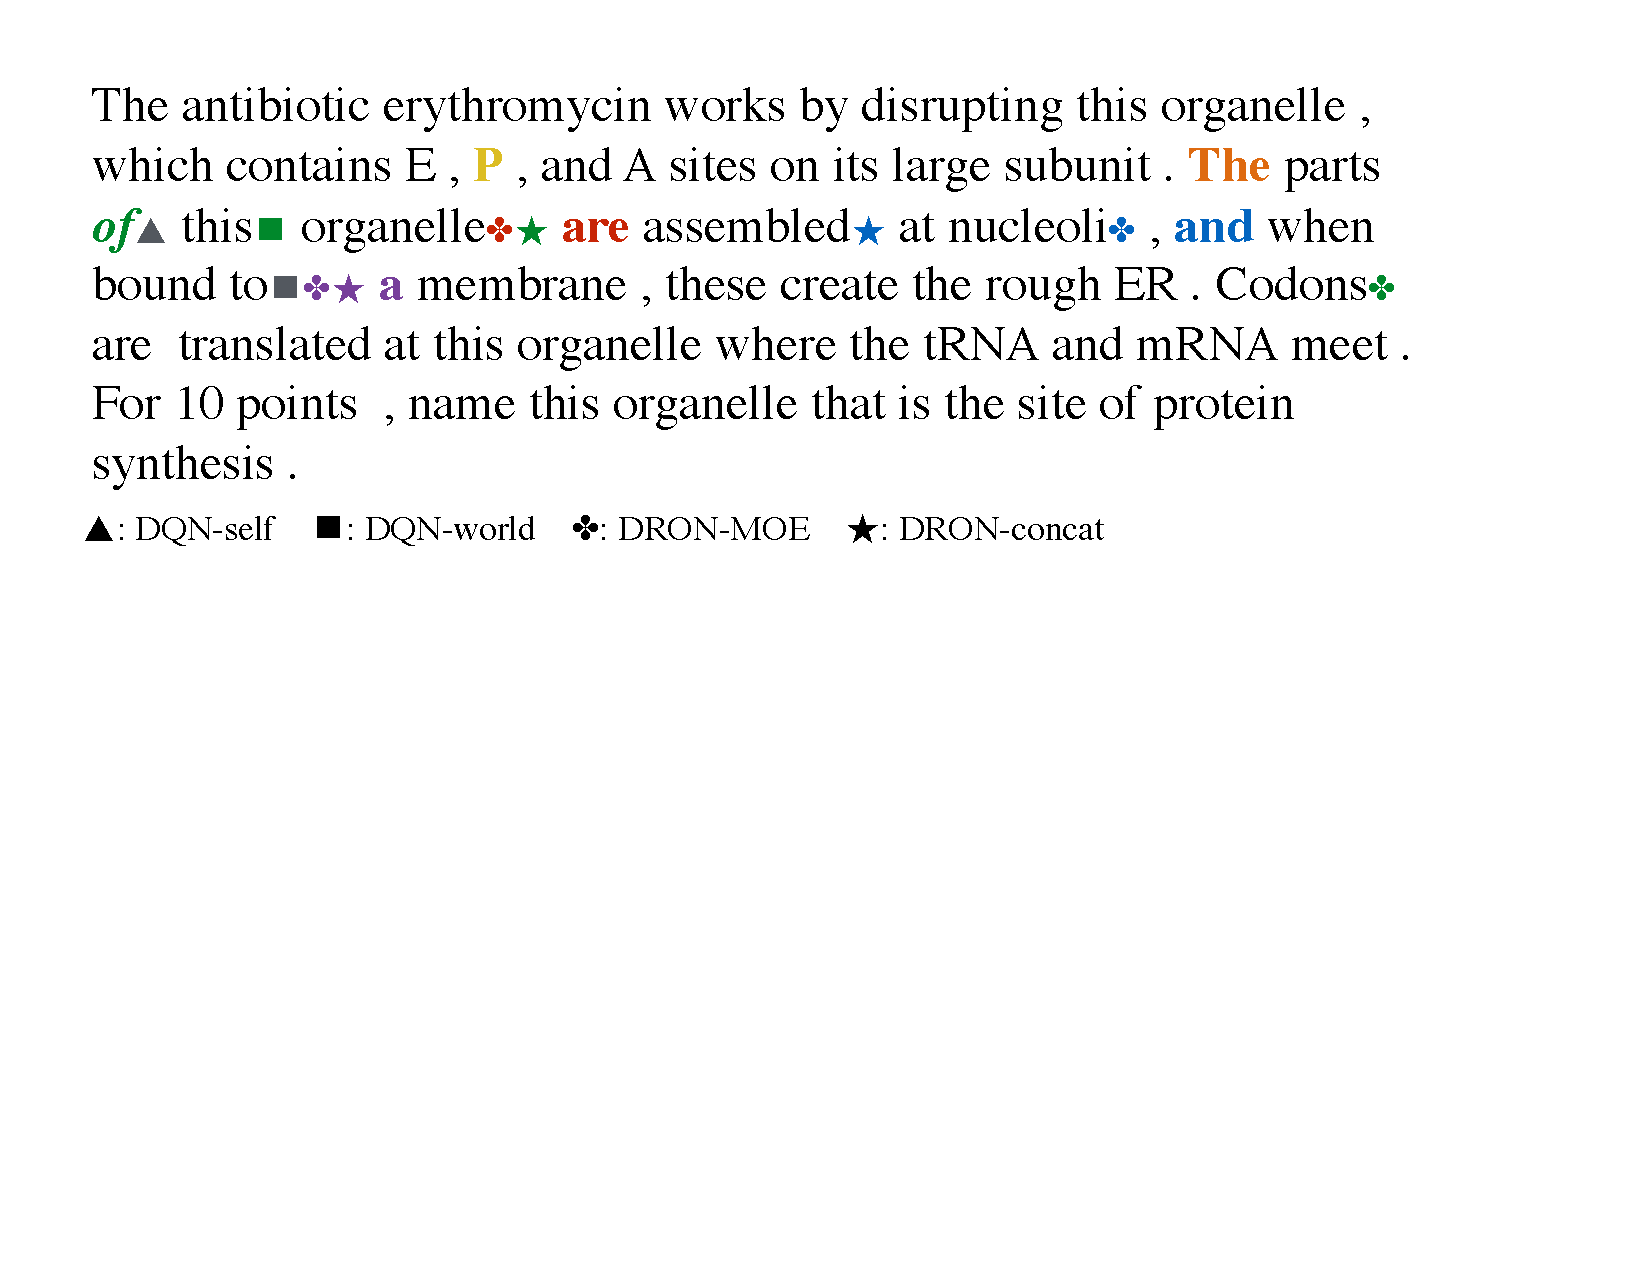
\includegraphics[width=1.0\columnwidth]{2016_icml_opponent/figures/qb_buzz_example}
\caption{Buzz positions of human players and agents on one science question whose answer is ``ribosome''.
Words where a player buzzes is displayed in a color unique to the player;
a wrong buzz is shown in \emph{italic}.
Words where an agent buzzes is subscripted by a symbol unique to the agent;
color of the symbol corresponds to the player it is playing against.
A gray symbol means that buzz position of the agent does not depend on its opponent.
\dron{} agents adjust their buzz positions according to the opponent's buzz position and correctness.
Best viewed in color.}
\label{fig:buzz_example}
\end{figure}

To investigate strategies learned by
these models, we show their performance against different types of players (as
defined at the end of ``Implementation'') in Table~\ref{tab:model_result}, right
column.  We compare three measures of
performance, the average reward ($R$), percentage of early and incorrect buzzes
(rush), and percentage of missing the chance to buzz correctly before the
opponent (miss).


All models beat Type~2 players, mainly
because they are the majority in our dataset.  As expected, \dqn{}-self learns a
safe strategy that tends to buzz early.  It performs the best against Type~1
players who answer early.  However, it has very high rush rate against cautious
players, resulting in much lower rewards against Type~3 and Type~4 players.  Without
opponent modeling, \dqn{}-world is biased towards the majority player, thus having
the same problem as \dqn{}-self when playing against players who buzz late.  Both
\dron{} models exploit cautious players while
holding their own against aggressive players.
Furthermore, \dronmoe{} matches \dqn{}-self against Type~1 players,
thus it discovers different buzzing strategies.

Figure~\ref{fig:buzz_example} shows an example question with buzz positions labeled.
The \dron{} agents demonstrate dynamic behavior against different players;
\dronmoe{} almost always buzzes right before the opponent in this example.
In addition, when the player buzzes wrong and the game continues, \dronmoe{} learns to wait longer since the opponent is gone, while the other agents are still in a rush.

As with the Soccer task,
adding extra supervision does not yield better results over \dronmoe{}
(Table~\ref{tab:model_result}) but significantly improves
\dron{}-concat.




Figure~\ref{fig:qb_moe_bar} varies the number of experts in \dronmoe{}
($K$) from two to four.  Using a mixture model for the opponents
consistently improves over the \dqn{} baseline, and using three
experts gives better performance on this task.  For multitasking,
adding the action supervision does not help at all.  However, the more
high-level type supervision yields competent results, especially with
four experts, mostly because the number of experts matches the
number of types.

\begin{figure}
\centering
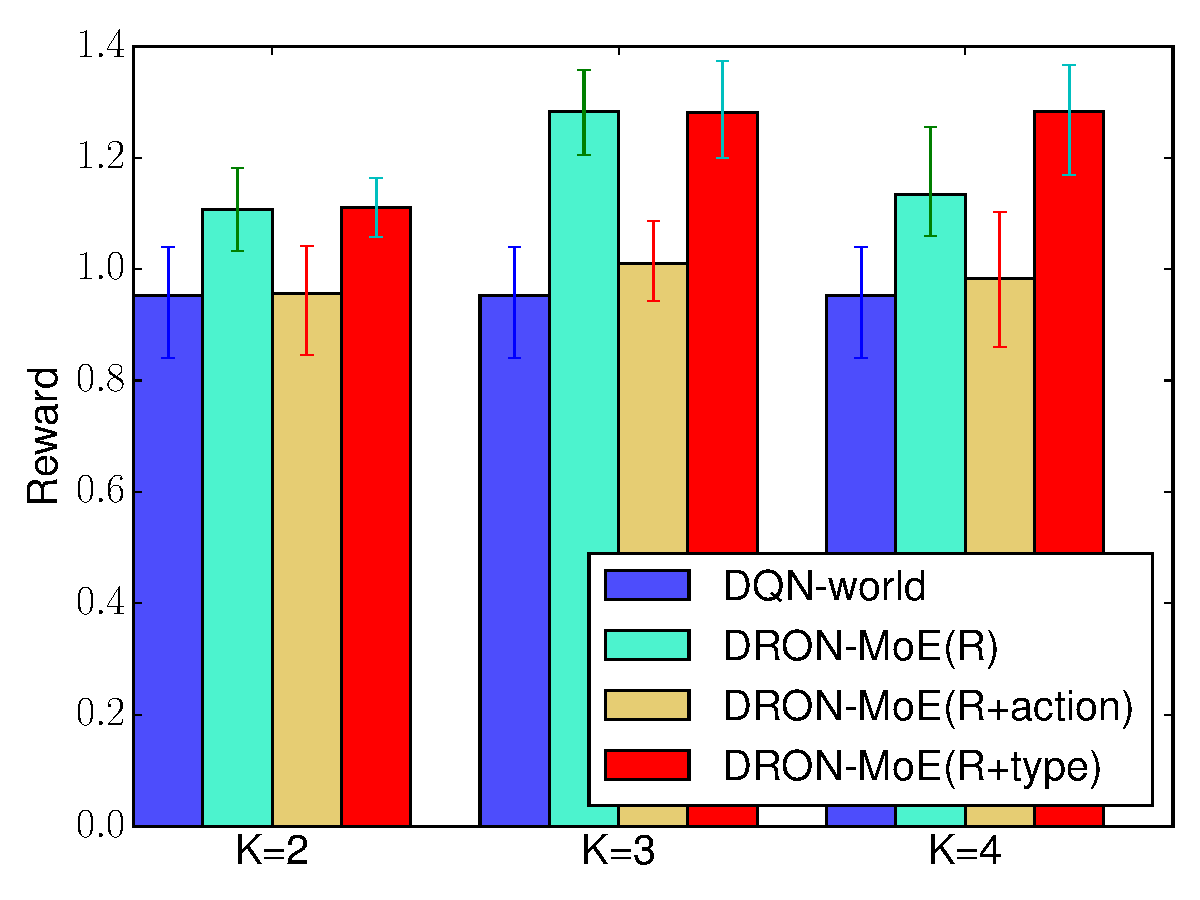
\includegraphics[width=0.6\linewidth]{2016_icml_opponent/figures/qb_moe_bar}
\caption{Effect of varying the number experts (2--4) and multitasking on quiz bowl.  The
  error bars show the 90\% confidence interval.  \dronmoe{} consistently
  improves over \dqn{} regardless of the number of mixture components.
  Supervision of the opponent type is more helpful than the specific
  action taken.  }

\label{fig:qb_moe_bar}
\end{figure}

\begin{figure}
\centering
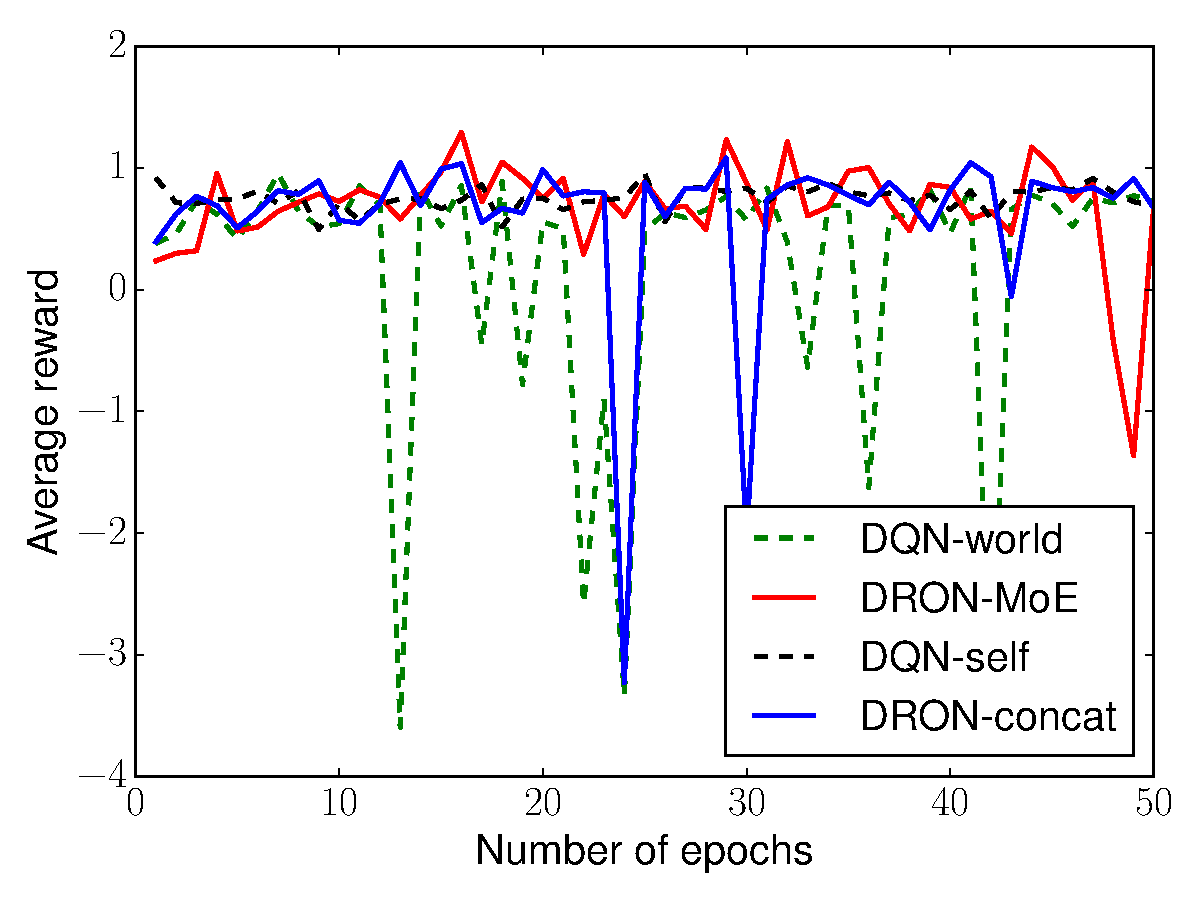
\includegraphics[width=0.6\linewidth]{2016_icml_opponent/figures/qb_all_test_rewards}
\caption{Learning curves on Quizbowl over fifty epochs. \dron{} models are more
  stable than \dqn{}.}
\label{fig:qb_all_test_rewards}
\end{figure}